\section{Experiments}
\label{sec:experiments}

We study the following questions
\begin{itemize}
\item
Scaling: how well does \algo{} scale to large networks? How effective are the techniques for choosing the
number of samples and pruning?
\item
Approximation Guarantees: what is the approximation factor of \algo{} in practice? How does it compare with 
the current best methods for intervention design in networks?
\item
Effect of multiple stages: how does the effectiveness of the solution vary with the number of stages
and the budget in each?
\item
Characteristics of the solutions: what kinds of nodes are picked in the solutions at each stage?
\end{itemize}

\subsection{Dataset and Methods}

\noindent
\textbf{Datasets.}
We experiment with three different classes of networks (total of five),
in order to fully explore the effect of network structure on the the results. 
We consider two random networks, namely the small world 
\cite{Kleinberg00thesmall-world}, and preferential attachment \cite{Barabasi509} models. 
We also consider synthetic agent based populations for Montgomery County, VA, and Portland, OR,
constructed by a first principles approach by \cite{barrett:wsc09,eubank:nature04}. This has been used in several public health studies, e.g., \cite{singh:bmc19}. This network has a rich set of demographic attributes for each node, e.g., age, gender, and income.
The datasets are summarized in Table \ref{tab:datasets}.

\noindent
\textbf{Choosing parameters.}
There is a large space of model parameters over which the analysis could be done. Due to the space limits, and
in order to get the most insights, we choose a subset as descirbed here.
We choose the source distribution $\src$ so that about 10 initial infections are picked.
Following standard practice in public health, e.g., \cite{halloran:pnas08},
we choose three values for the transmission probability $p$ based on the expected number of infections (referred to as the ``attack rate'') 
that result when there are no interventions: we choose a probability $p_{low}$ if the attack rate is $<10\%$ (low),
$p_{med}$ if the attack rate is in $[10\%, 20\%]$ (medium), and
$p_{high}$ if the attack rate is $> 20\%$.
The specific probability values depend on the datasets.
The full version of the paper \cite{fullversion} shows how the attack rate varies with the probability,
and the specific probability values which were chosen.



\begin{table}[!h]
\centering
\begin{tabular}{llll}
\hline
 \textbf{Dataset} & \textbf{Nodes} & \textbf{Edges}   \\ \hline
 Montgomery & 70729 & 198138 \\
 Portland & 1409197 & 8307767 \\
 Small World (SW) & 2500 & 14833 \\   
 Preferential1 (PA1) & 1000 & 1996 \\ 
Preferential2 (PA2) & 100000 & 199996 \\ \hline
\end{tabular}
\caption{Description of datasets}
\label{tab:datasets}
\end{table}

\noindent
\textbf{Methods.}
We only focus on one stage (\probone) or two stage (\probtwo) versions of \prob{} here, and use \algo{} to find 
interventions. We use the Gurobi solver to implement \algo{}.
For \probone{}, we consider the following baselines, which select $B$ nodes based on two criteria:
\begin{itemize}
\item
Nodes with the highest degree, which has been a popular approach in a number of papers
\cite{salathe:plos12, Barabasi509}
\item
Nodes with the highest eigenscore: this, and its variants have been shown to be the best strategy to reduce the spectral radius
\cite{tong:cikm12,zhang2015controlling,YaoSDM2014,AAAI1816714,PreciadoVM13_2,PreciadoVM13,PreciadoVM14}
\end{itemize}

No prior results are known for \probtwo{}. Therefore, we adapt the above baselines and pick $B_0$ and $B_T$
nodes in the order of the above scores.


\subsection{Scaling}

We find that \algo{} easily scales to all the networks we consider. The two strategies for speeding up have a
significant impact on the scaling.
\begin{itemize}
\item
Number of samples needed: we find $O(\sqrt{n})$ samples are sufficient to get reasonable variance, as shown in Figure \ref{fig:pa_boxplot},
instead of the worst case bound of $\Theta(n\log{n})$ from Lemma \ref{lemma:conc}.
The number of samples needed is lower when the transmission probability is medium or high, and when the budget is not too high,
since this has better convergence. We note that these are typically the regimes of maximum concern in public health.
\item
Impact of pruning: the pruning of low vulnerability nodes has a very significant impact on the running time,
as shown in Figure \ref{fig:pa1pruningtime}, which shows the running time with and without pruning. 
When the number of samples used is low, the difference is negligible, but when the number of samples increases to
the range needed for low variance, we find the difference in running time is several orders of magnitude.
The objective value differs by less than $5\%$ with and without pruning, as shown in Figure \ref{fig:pa1pruningobj}.
This implies that our scaling strategies give good solutions on very large networks.
\end{itemize}
 
\begin{figure}[!h]
    \centering
    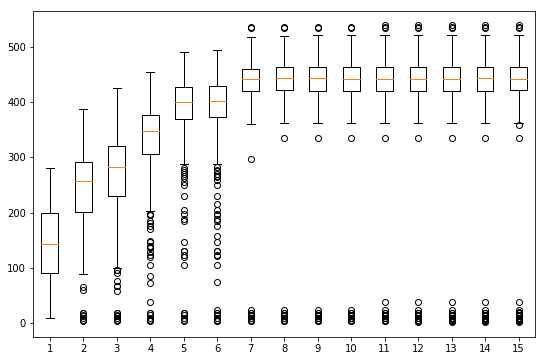
\includegraphics[scale = 0.4]{Figuresnew/boxplotpa.png}
    \caption{Average number of infections over the $M$ samples (y-axis) vs $M/100$, i.e., the number of samples (in 100s) on the x-axis
for the Preferential Attachment (PA2) network.
}
    \label{fig:pa_boxplot}
\end{figure}


\begin{figure}[!h]
    \centering
    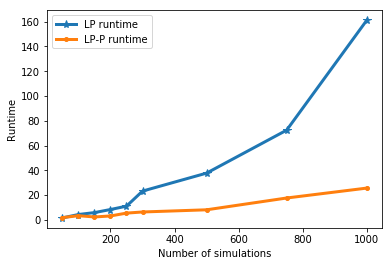
\includegraphics[scale = 0.55]{Figuresnew/pa1_runtime.png}
    \caption{Comparison of runtimes of Linear Programs with (LP-P) and without pruning (LP) on y-axis vs 
number of samples on x-axis for the PA1 network. }
    \label{fig:pa1pruningtime}
\end{figure}
\subsection{Performance Guarantees}
Will have plots for the larger datasets for both comparison with baselines and approximation guarantees.



\begin{figure}[!h]
    \centering
    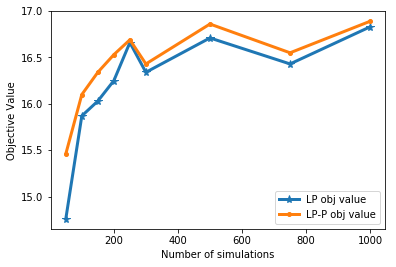
\includegraphics[scale = 0.55]{Figuresnew/pa1_objpruning.png}
    \caption{Comparison of the objective values of Linear Programs with (LP-P) and without pruning (LP) on the y-axis
vs the number of samples on the x-axis for the PA1 network. }
    \label{fig:pa1pruningobj}
\end{figure}

\subsection{Performance Guarantees}
Will have plots for the larger datasets for both comparison with baselines and approximation guarantees.

\subsubsection{Comparison to baselines}
\subsubsection{Approx Ratio}
\begin{figure}[!h]
    \centering
    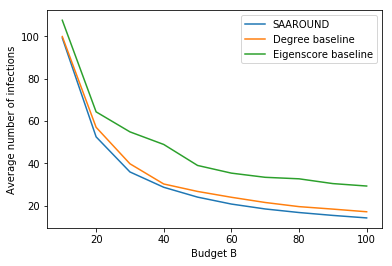
\includegraphics[scale = 0.55]{Figuresnew/pa1_obj.png}
    \caption{Preferential1: Comparison of \algo{} with the degree and eigenscore based baselines.}
    \label{fig:pa1approx}
\end{figure}

\begin{figure}[!h]
    \centering
    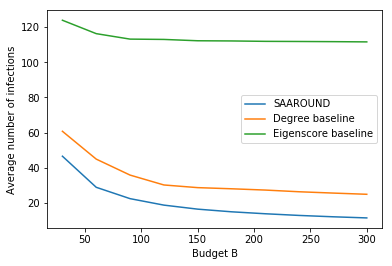
\includegraphics[scale = 0.55]{Figuresnew/pa2_obj.png}
    \caption{Preferential2: Comparison of \algo{} with the degree and eigenscore based baselines.}
    \label{fig:pa1approx}
\end{figure}

\begin{figure}[!h]
    \centering
    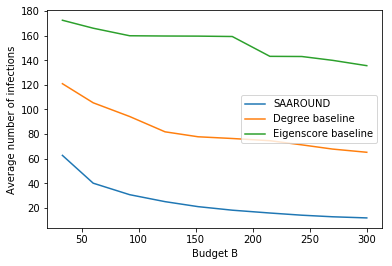
\includegraphics[scale = 0.55]{Figuresnew/mont_obj.png}
    \caption{Montgomery: Comparison of \algo{} with the degree and eigenscore based baselines.}
    \label{fig:pa1approx}
\end{figure}
\subsection{Two stage intervention and Structure of solution}
We study the two stage version of \prob{}. Here no information about the outbreak is available, and so, clearly, earlier is better, i.e., if the entire budget is available at time $0$, it is better to use it right away. In Figure \ref{fig:temporal}, we examine how the objective value $\expinf{}$ increases with $T$ in a two stage intervention, where $T$ is the time of the second stage. We observe that $\expinf{}$ increases very rapidly with $T$.

Next, we examine the structure of the sets picked in each stage. Figure \ref{fig:montagedeg} shows a scatter plot of the node degree and age of the solution to a two stage version with $T=4$. We observe that there are slight differences between the sets $X_0$ and $X_4$: $X_0$ has slightly higher degree nodes, whereas $X_4$ has slightly lower age nodes. But more importantly, \emph{it is not the case that all high degree nodes are used in $X_0$}.
\begin{figure}[!h]
    \centering
    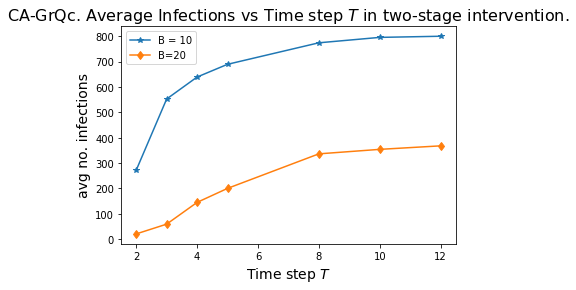
\includegraphics[scale = 0.45]{figures/twostage.png}
    \caption{CA-GrQc. Impact of varying $T$ in Two-stage Intervention. The X-axis corresponds to time step $T$ at which 2nd intervention is performed (1st intervention is at T =0). The Y-axis corresponds to the average number of infections over the simulations.}
    \label{fig:temporal}
\end{figure}

\begin{figure}[!h]
    \centering
    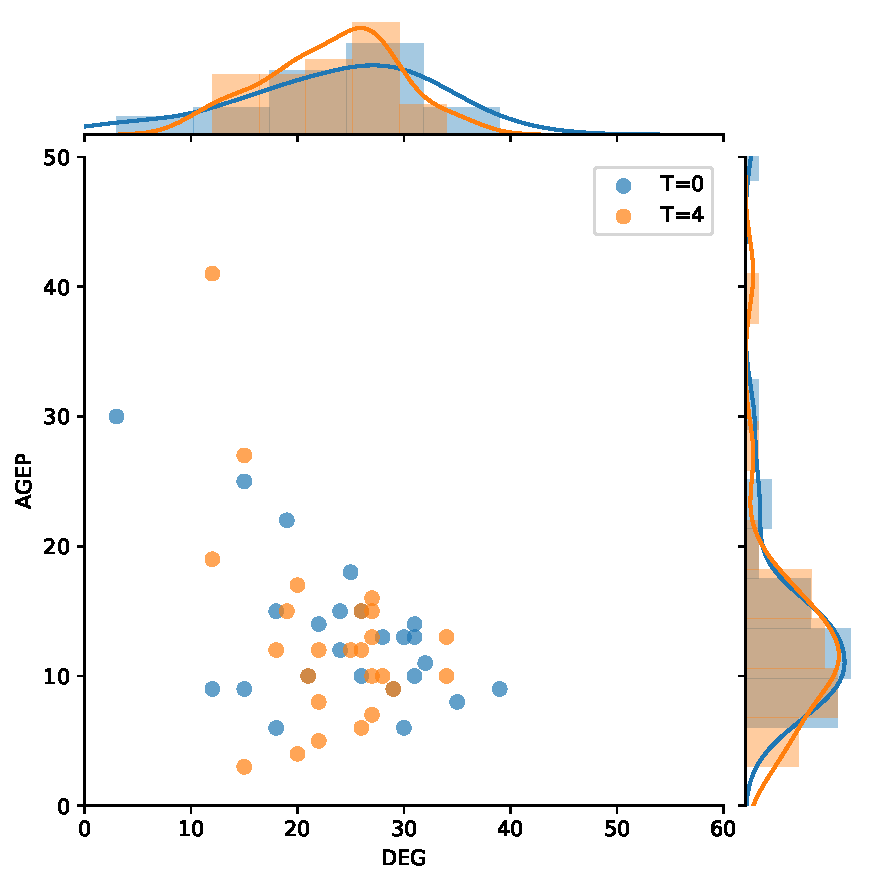
\includegraphics[scale = 0.45]{figures/t0_t4_compare_age_deg.pdf}
    \caption{Montgomery Graph: scatter plot of age and degree of nodes of the sets $X_0$ and $X_4$ in a solution to the 2-stage \prob{} with budgets $B_1 = B_4 = 25$.}
    \label{fig:montagedeg}
\end{figure}

\
%\subsection{Approximation Guarantees}


%\subsection{Characterizing Structure of Solution}

